\chapter{Friedmann-Gleichung\label{chapter:thema}}
\lhead{Friedmann-Gleichung}
\begin{refsection}
\chapterauthor{Andri Hartmann und Tobias Schuler}
\printbibliography[heading=subbibliography]
\section{Expansion des Universums}
Seit langem stellte man sich die Frage, was das Universum ist und wie es sich verh"alt. Als 1912 Albert Einstein die Relativit"atstheorie herleitete, konnten gewisse Fragen beantwortet werden.
%\subsection{Kosmologische Rotverschiebung}
%Die Kosmologische Rotverschiebung ist nicht zu verwechseln mit dem Dopplereffekt. Grund daf\"{u}r ist, dass sich die Galaxien nicht in der Raumzeit voneinander entfernen, sondern sich der Raum ausdehnt. 
\subsection{Alexander Friedmann und Georges Lema\^{i}tre}
Beide entdeckten im Jahre 1927 unabh"angig voneinander die Friedmann-Lema\^{i}tre-Gleichung. Diese beschreibt das Verhalten des Universums seit dem Urknall. 
\begin{equation}
\left(\frac{a'}{a}\right) ^2 = \frac{8 \pi G}{3} \rho - \frac{k c^2}{a^2} + \frac{\Lambda c^2}{3}
\end{equation}
\subsubsection{Herleitung der Gleichung}
Um das Universum wird ein Raster gelegt. Die Einheit des Rasters wird durch den Skalenfaktor $a$ ausgedr"uckt. Der Skalenfaktor ist abh"angig von der Zeit. Ver"andert sich das Raster, ver"andern sich auch die Positionen der Sterne und Galaxien.
%\begin{figure}
%	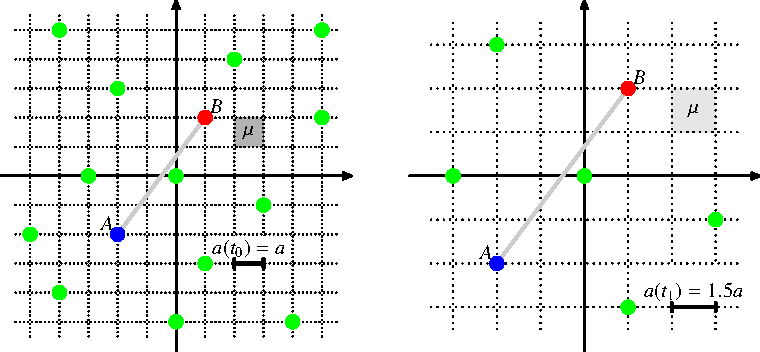
\includegraphics[width = \textwidth ]{chapters/images/friedmann-1.png}
%\end{figure}
Die Distanz zwischen Punkt A und Punkt B entspricht 
\begin{equation}
D_{AB} = \sqrt{a^2(t)\Delta_{AB}x^2 + a^2(t)\Delta_{AB}y^2 + a^2(t)\Delta_{AB}z^2} = a(t) \sqrt{\Delta_{AB}x^2 + \Delta_{AB}y^2 + \Delta_{AB}z^2}
\end{equation}
F\"{u}r die Geschwindigkeit, mit der sich die beiden Punkte voneinander wegbewegen, gilt 
\begin{equation}
v_{AB} = \dfrac{dD_{ab}}{dt} 
	   = a'(t) \sqrt{\Delta_{AB}x^2 + \Delta_{AB}y^2 + \Delta_{AB}z^2}
\end{equation}
Dabei sieht man, dass sich der Abstand in x-, y- und z-Richtung nicht ver\"{a}ndert hat und konstant bleibt. Um von diesem Abstand wegzukommen, wird die Geschwindigkeit durch die Distanz geteilt.
\begin{equation}
\frac{v_{AB} }{D_{AB}} = \frac{a'(t)}{a(t)}
\label{friedmann:geschwindigkeit}
\end{equation}
\begin{satz} [Hubble-Konstante]
	Die Ableitung des Skalenfaktors dividiert durch den Skalenfaktor entspricht der Hubble-Konstante.
	\[
	\frac{a'(t)}{a(t)} = H
	\]
\end{satz}
Wir gehen von einem homogenen Universum aus, was bedeutet, dass die Masse gleich verteilt ist. Die Masse im W"urfel mit Dimension $\Delta x$, $\Delta y$ und $\Delta z$ ist 
\begin{equation}
M_{xyz} = \nu \Delta x \Delta y \Delta z
\end{equation}
wobei $\nu$ eine Konstante ist. Sie beschreibt die Masse im W"urfel f"ur eine bestimmte Gr"osse. Das Volumen des W"urfels ist bekanntlich 
\begin{equation}
V_{xyz} = a^3 \Delta x \Delta y \Delta z
\end{equation}
Die Dichte im W"urfel ist  
\begin{equation}
\rho = \frac{M_{xyz}}{V_{xyz}} = \frac{\nu}{a^3}
\label{friedmann:dichte}
\end{equation}
\subsubsection{Beschleunigung des Skalenfaktors}
Setzt man eine Masse M in den Ursprung des Skalenfaktor-Koordinatensystems, gelten folgende physikalische Regeln f"ur die Masse m 
\[D =  a(t) \sqrt{\Delta x^2 + \Delta y^2 + \Delta z^2}  = a(t) R\]
\[v = a'(t) R\]
\[A = a''(t) R\]
\[V = \frac{4 \pi }{3} R^3\]
D steht f"ur die Distanz zwischen m und M, v f"ur die Geschwindigkeit, A f"ur die Beschleunigung und V f"ur das Volumen der Kugel mit Radius R. Newton hat bewiesen, dass alle Masse innerhalb der Kugel mit Radius D im Ursprung als Punktmasse M angenommen werden kann. Die Masse ausserhalb der Kugel hat keine Einwirkung. Daraus ergibt sich die Gravitationskraft
\begin{equation}
F_G = -\frac{m M G}{D^2}
\end{equation}
Da die Gravitationskraft zwecks Vereinfachung des Modells als einzige Kraft eingesehen wird, gilt f"ur die Beschleunigung mit 
\[F = m A\]
\[A = - \frac{M G}{D^2} = a'' R \Rightarrow a''(t) = \frac{- M G}{a^2 R^3} \Rightarrow\ \frac{a''(t)}{a} = \frac{-\frac{4 \pi }{3} M G}{\frac{4 \pi}{3}a^3 R^3} \Rightarrow \frac{a''(t)}{a} = \frac{- 4 \pi G}{3} \frac{M}{V}\]
Die Gleichung wurde so angepasst, dass oben die Masse und unten das Volumen steht. Damit vereinfacht sich die Beschleunigung zu
\begin{equation}
\frac{a''(t)}{a} = \frac{- 4 \pi G}{3} \rho
\end{equation}
\subsubsection{Bedeutung der Beschleunigungsgleichung}
Setzt man f"ur die Dichte Gleichung \ref{friedmann:dichte} ein ergibt sich
\[\frac{a''(t)}{a} = \frac{- 4 \pi G}{3} \frac{\nu}{a^3} \Rightarrow \frac{a''(t)}{a} = \frac{- 4 \pi G \nu}{3} \frac{1}{a^3}\]
Der erste Term auf der rechten Seite der Gleichung entspricht mehreren Konstanten, welche wir durch die Konstante $c$ ersetzen. So vereinfacht sich die Gleichung zu
\[\frac{a''}{a} = \frac{c}{a^3} \Rightarrow a'' = \frac{c}{a^2}\]
Die Differentialgleichung ist nichtlinear und mit MatLab nicht l"osbar. Trotzdem k"onnen wir gewisse Aussagen machen, n"amlich
\begin{enumerate}
	\item Die Beschleunigung wirkt der Ausdehnung des Universums entgegen. Sie ist negativ, weil $c$ eine negative Konstante ist  und $a^2$  immer positiv ist. 
	\item Eine negative Beschleunigung bedeutet aber nicht, dass sich das Universum verkleinert.
\end{enumerate}

\subsubsection{Energieerhaltung}
Die Energie der Masse $m$ besteht aus kinetischer und potentieller Energie.
\begin{equation}
E_m = E_{kin} - E_{pot} =  \frac{m v^2}{2} - \frac{m M G }{x}, \qquad x = \text{Abstand zwischen der Masse M und m}
\end{equation}
Dabei k"onnen drei F"alle auftreten, n"amlich
\begin{enumerate}
	\item $E_m > 0 \rightarrow$ Die Masse $m$ kann nicht umkehren, der Term der kinetischen Energie "uberwiegt.
	\item $E_m = 0 \rightarrow$ Die Masse $m$ kommt auf einer gewissen H"ohe zum Stillstand. (Escape Velocity)
	\item $E_m < 0 \rightarrow$ Die Masse $m$ wird so stark angezogen, dass die Geschwindigkeit ihre Richtung "andert.
\end{enumerate}
Wir setzen $E_m = 0$ und formulieren um. Danach wenden wir die Gesetze unseres 'Raster-Universum' an, indem wir $v_a_b$ und $D_a_b$ einsetzen.
\[\frac{m v^2}{2} = \frac{m M G}{x} \qquad| *\frac{2}{m} \qquad \Rightarrow {v^2} = \frac{2 M G}{x}\]
\[\left(a'(t) \sqrt{\Delta_{AB}x^2 + \Delta_{AB}y^2 + \Delta_{AB}z^2}\right)^2 = \frac{2 M G}{a(t)\sqrt{\Delta_{AB}x^2 + \Delta_{AB}y^2 + \Delta_{AB}z^2}}}\] 
Den Abstand zwischen $m$ und $M$ normieren wir auf eins.
\[a'(t)^2 = \frac{2 M G}{a(t)}\] 
\end{refsection}

